\documentclass[a4paper,12pt]{article}

% No intetation
\usepackage[parfill]{parskip}

% Calligraphic math
% \usepackage{calrsfs}
% \usepackage{boondox-cal}

\usepackage{amsmath}
\DeclareMathOperator*{\argmin}{\arg\!\min}
\newcommand{\argminUnder}{\arg\!\min}
\usepackage{mathtools}
\DeclarePairedDelimiter\abs{\lvert}{\rvert}
\DeclarePairedDelimiter\norm{\lVert}{\rVert}

% R symbol
\usepackage{amssymb}
\newcommand{\R}{\mathbb{R}}

% For bold
\usepackage{bm}

% Font
\usepackage{fontspec}
\setmainfont{GFS Artemisia}

% English-Greek use
\usepackage{polyglossia}
% \setmainlanguage{english}
% \setotherlanguage{greek}
\setmainlanguage{greek}
\setotherlanguage{english}

\iffalse
\usepackage[greek, english]{babel}
\fi

\newfontfamily\greekfont{GFS Artemisia}
\let\greekfonttt\ttfamily

% Hyperlinks
\usepackage[hidelinks, pdfencoding=auto]{hyperref}
\renewcommand{\figureautorefname}{Σχήμα}

% Images
\usepackage{graphicx}
\graphicspath{{./images/}}
\usepackage[font={footnotesize,it}]{caption}
\usepackage[font={footnotesize}]{subcaption}
\renewcommand{\thesubfigure}{\Roman{subfigure}}

% New page every section
\usepackage{titlesec}
\newcommand{\sectionbreak}{\clearpage}

% References
\usepackage[backend=biber,style=ieee]{biblatex}
\addbibresource{references.bib}
% \bibliography{references} 

\usepackage[justify]{ragged2e}
% \justifying


\tolerance=10000 
% \pretolerance=10000

\begin{document}

\tableofcontents

\listoffigures

\section{Εισαγωγή}

\subsection{Διατύπωση του προβλήματος}

Η κατάτμηση είναι η διαδικασία διαμέρισης μίας εικόνας σε διάφορα ουσιαστικά
τμήματα. Σκοπός της κατάτμησης είναι η απλοποίηση ή/και η αλλαγή της
αναπαράστασης της εικόνας σε κάτι που είναι πιο σημασιολογικά σημαντικό και
είναι πιο εύκολο να αναλυθεί. Πιο συγκεκριμένα, η κατάτμηση εικόνας είναι η
διαδικασία ανάθεσης μίας ετικέτας σε κάθε εικονοστοιχείο της εικόνας έτσι ώστε
τα εικονοστοιχεία με την ίδια ετικέτα να έχουν ίδια χαρακτηριστικά.

Στην ιατρική απεικόνιση αυτά τα τμήματα αντιστοιχούν συχνά σε διαφορετικές
κατηγορίες ιστών, οργάνων, παθολογίες ή άλλες βιολογικά σχετιζόμενες δομές. Η
αυτοματοποιημένη κατάτμηση ιατρικών απεικονίσεων μπορεί να βοηθήσει τους
γιατρούς επιταχύνοντας τη διαδικασία διάγνωσης. Η καθημερινή δημιουργία πληθώρας
ιατρικών απεικονίσεων καθιστά τη χειροκίνητη κατάτμηση από ειδικούς όλο και
δυσκολότερη, λόγο του χρονικού διαστήματος που χρειάζεται η ανάλυση. Επομένως, η
ανάπτυξη αξιόπιστων, σταθερών και ακριβών τεχνικών για την αυτοματοποιημένη
κατάτμηση ιατρικών απεικονίσεων αποτελεί μία σημαντική πρόκληση.

\subsubsection{Κατάτμηση βάση ατλάντων}

Η κατάτμηση απεικονίσεων βάση ατλάντων αποτελεί την διαδικασία κατά την οποία
χρησιμοποιούνται απεικονίσεις που έχουν κατανεμηθεί από κάποιον ειδικό, ούτως
ώστε να επιτευχθεί η κατάτμηση της νέας απεικόνισης. Οι μέθοδοι αυτοί συνήθως
απαιτούν την χρήση καταχώρησης εικόνας (image registration) με σκοπό την
ευθυγράμμιση τού ή των ατλάντων στην εικόνα-απεικόνιση που πρόκειται να
κατανεμηθεί.

\subsubsection{Αντικείμενο διπλωματικής εργασίας}

Στην διπλωματική εργασία εφαρμόστηκαν μέθοδοι κατάτμησης ιατρικών απεικονίσεων
βάση ατλάντων με χρήση μηχανικής μάθησης. Οι απεικονίσεις αφορούν μαγνητικές
τομογραφίες σε γόνατα και οι περιοχές κατάτμησης αποτελούνται από τους αρθρικούς
χόνδρους και τα οστά. Τα δεδομένα που χρησιμοποιήθηκαν προέρχονται από το
Osteoarthritis Initiative Zuse Institute Berlin(OAI ZIB). Οι μέθοδοι που
χρησιμοποιήθηκαν προέρχονται από μεθόδους που έχουν χρησιμοποιηθεί για την
κατάτμηση περιοχών του εγκεφάλου.
TODO: references


\section{Θεωρητικό υπόβαθρο}

\subsection{Πλαίσιο συγχώνευσης κατηγοριών βασισμένο σε γράφους}

Το πλαίσιο συγχώνευσης κατηγοριών βασισμένο σε γράφους προτάθηκε από
το \cite{Zhang:1} ως μία μέθοδος μέσω της οποίας μπορούν να παραχθούν πολλές
υπάρχουσες μέθοδοι συγχώνευσης κατηγοριών.

Έστω το ζεύγος $\{(I_i,L_i),i=1,...,n\}$ όπου $I_i$ είναι η απεικόνιση ενός
άτλαντα, $L_i$ ο χάρτης των κατηγοριών της αντίστοιχης απεικόνισης και $n$ το
σύνολο των ατλάντων. Δοθείσας μία απεικόνισης $I$, δημιουργείται ο γράφος $G_i$
μεταξύ των εικονοστοιχείων $\bm{x}$ της δοθείσας εικόνας $I$ και του
εικονοστοιχείου $\bm{y}$ της απεικόνισης του άτλαντα $I_i$, μαζί με τα
αντίστοιχα βάρη $w_i(\bm{x},\bm{y})$, για $(\bm{x},\bm{y})\in\Omega^2$, όπου
$\Omega$ ο χώρος των απεικονίσεων. Με τη δημιουργία των βαρών του γράφου, η
συγχώνευση των κατηγοριών γίνεται για κάθε $\bm{x}$ της απεικόνισης εισόδου $I$
σύμφωνα με το τύπο:

\begin{equation}
    L(\bm{x})=\frac{ \sum_{i=1}^{n}  \sum_{\bm{y}\in\Omega}
                     w_i(\bm{x},\bm{y})L_i(\bm{y})}
    { \sum_{i=1}^{n}  \sum_{\bm{y}\in\Omega} w_i(\bm{x},\bm{y}) }
    , \forall \bm{x}\in\Omega
\end{equation}

$L$ είναι ο χάρτης των κατηγοριών της απεικόνισης εισόδου $I$.

% Lasso
\subsection{Ελάχιστα απόλυτος τελεστής συρρίκνωσης και επιλογή}

Ο ελάχιστα απόλυτος τελεστής συρρίκνωσης και επιλογής (least absolute shrinkage
and selection operator, Lasso) \cite{Lasso:1} είναι μία μέθοδος παλινδρόμησης.
Παλινδρόμηση είναι η μέθοδος πρόβλεψης της συμπεριφοράς μίας μεταβλητής
βασισμένη σε μία ή περισσότερες άλλες μεταβλητές. Έστω οι παρατηρήσεις
$(\bm{x_i},y_i), i=1,...,N$, όπου $\bm{x_i}=(x_{i1},...,x_{ip})$ οι $p$
μεταβλητές εισόδου και $y_i$ η μεταβλητή εισόδου για την $i$-οστή παρατήρηση. Αν
$\hat{\beta} = (\hat{{\beta}_1},...,\hat{{\beta}_p})^T$ και $\hat{\alpha}$ τα
αποτέλεσματα της παλινδρόμησης (συντελεστές παλινδρόμησης) τότε ο τελεστής
ορίζεται ως:

\begin{equation}\label{lassoEq1}
    (\hat{\alpha}, \hat{\beta}) = 
    \argmin{\left\{\sum_{i=1}^{N} {\left(\,y_i-\alpha- \sum_{j=1}^{p}
    \beta_{j}x_{ij}\right)}^2 \right\}} 
    \text{ subject to }
    \sum_{j=1}^{p} \abs{\beta_j} \leq t
\end{equation}

Το $t \geq 0$ είναι παράμετρος συντονισμού. Για κάθε τιμή του $t$ η λύση για το
$\alpha$ είναι $\hat{\alpha}=\overline{y}$ (όπου $\overline{y}$ είναι η μέση
τιμή του $y$). Επίσης μπορούμε να υποθέσουμε χωρίς την απώλεια της γενίκευσης
ότι $\hat{\alpha}=0$ ώστε να εξαλειφθεί το $\alpha$. Έστω $\bm{X} =
(\bm{x_1},...,\bm{x_N})^T$ και $y = (y_1,...,y_N)^T$ τότε η \eqref{lassoEq1}
μπορεί να γραφτεί ως:

\begin{equation}\label{lassoEq2}
    \hat{\beta} = 
    \argmin{\left\{\frac{1}{N} \norm{\left(\,y - \bm{X} \beta\right)}_2^2
    \right\}} 
    \text{ subject to }
    \norm{\beta}_1 \leq t
\end{equation}

Όπου η $p$-οστή νόρμα του $x=(x_1,...,x_n)$ ορίζεται ως:

\begin{equation*}
    \norm{x}_p=\left( \sum_{i=1}^{n} \abs{x_i}^p\right)^{1/p}
\end{equation*}

Η εξίσωση \eqref{lassoEq2} μπορεί να γραφτεί επίσης με την χρήση του
πολλαπλασιαστή Lagrange ως:

\iffalse
Όπου $\norm{x}_p=\left( \sum_{i=1}^{n} \abs{x_i}^p\right)^{1/p}$ είναι η
$p$-οστή νόρμα του $x=(x_1,...,x_n)$. Η εξίσωση μπορεί να γραφτεί επίσης με την
χρήση του πολλαπλασιαστή Lagrange ως:
\fi

\begin{equation}\label{lassoEq3}
    \hat{\beta} = 
    \argmin{\left\{\frac{1}{N} \norm{\left(\,y - \bm{X} \beta\right)}_2^2 +
    \lambda \norm{\beta}_1 \right\}} 
\end{equation}

Πολλές φορές οι στήλες του $\bm{X}$ κανονικοποιούνται, δηλαδή ισχύει:

\begin{equation*}
    \sum_{j=1}^{p} {\frac{x_{ij}}{N}} = 0
    \text{ , }
    \sum_{j=1}^{p} {\frac{x_{ij}^2}{N}} = 1
\end{equation*}


\iffalse
% TODO: Ίσως να το ϐαλω αυτό:
Το πλεονέκτημα του ελάχιστα απόλυτου τελεστή συρρίκνωσης και επιλογής είναι ότι
σε σχέση 
TODO: least squares, why lasso 
\fi

% registration
\subsection{Καταχώρηση εικόνας}

Καταχώρηση εικόνας (image registration) είναι η διαδικασία μετασχηματισμού
διαφορετικών δεδομένων σε ένα σύστημα συντεταγμένων. Η διαδικασία αυτή επιδιώκει
μέσω του μετασχηματισμού αυτού, την επικάλυψη των κοινών χαρακτηριστικών των
δεδομένων. Τα δεδομένα μπορεί να είναι πολλαπλές φωτογραφίες, δεδομένα από
διαφορετικούς αισθητήρες, ώρες, βάθη και οπτικές \cite{Registration:1}. Στις
ιατρικές απεικονίσεις επιδιώκεται μέσω του μετασχηματισμού, αντίστοιχα
εικονοστοιχεία των απεικονίσεων να αναπαριστούν όμοια βιολογικά σημεία.

Συνήθως στις μεθόδους καταχώρησης εικόνας η μία εικόνα παραμένει σταθερή κατά
την διαδικασία της καταχώρησης και η άλλη-άλλες μετασχηματίζονται. Η εικόνα που
παραμένει σταθερή αποκαλείται εικόνα αναφοράς ή απλά σταθερή εικόνα. Οι εικόνες
που μετασχηματίζονται ονομάζονται εικόνες καταχώρισης ή κινούμενες εικόνες.

%TODO: εικόνα εδώ;

Η βασική διαδικασία της καταχώρησης εικόνας αποτελείται από την ανίχνευση
χαρακτηριστικών, την ευθυγράμμιση χαρακτηριστικών από την κινούμενη εικόνα στην
σταθερή, εκτίμηση παραμέτρων συναρτήσεων χαρτογράφησης, την δειγματοληψία και
τον μετασχηματισμό εικόνας. Οι μέθοδοι καταχώρισης εικόνας είναι μοναδικές για
κάθε πρόβλημα και δεν υπάρχει κοινή τεχνική καταχώρισης εικόνας που να είναι
ισάξια αποτελεσματική σε κάθε πρόβλημα που εφαρμόζεται \cite{Registration:2}.
Για παράδειγμα υπάρχουν μέθοδοι που βασίζονται στην ένταση των εικόνων και
μέθοδοι που βασίζονται σε χαρακτηριστικά τους.

% Οι μέθοδοι της καταχώρησης εικόνας διαφέρουν ανάλογα με το δεδομένα που
% πρόκειται να καταχωρηθούν \cite{Registration:2}. 

\subsubsection{Μέση διαφορά τετραγώνων} \label{MSSD}

Στην οικογένεια των μεθόδων που βασίζονται στην ένταση των εικόνων, η μέτρηση
της ομοιότητας μεταξύ της κινούμενης και της σταθερής εικόνας αποτελεί ένα
δομικό στοιχείο της καταχώρησης εικόνας. Η μέτρηση αυτή αξιολογεί την
καταλληλότητα του μετασχηματισμού και χρησιμοποιείται για να υπολογιστεί η
παράγωγος της αξιολόγησης, ούτως ώστε να χρησιμοποιηθούν από τον αλγόριθμο
βελτιστοποίησης. Η επιλογή της μετρικής βασίζεται στο εκάστοτε πρόβλημα που
επιχειρεί να λύσει

Η μέση διαφορά τετραγώνων υπολογίζει τον μέσο όρο των τετραγώνων της διαφορά της
έντασης για κάθε εικονοστοιχείο μεταξύ της σταθερής και της κινούμενης εικόνας.
Η μετρική αυτή βασίζεται στην υπόθεση ότι η ένταση όμοιων σημείων είναι η ίδια
και στις δύο εικόνες και έχει την ίδια κατανομή και στις δύο εικόνες. Αυτό
σημαίνει ότι και οι δύο εικόνες έχουν την ίδια μορφή. 

Η μέση διαφορά τετραγώνων ορίζεται ως:

\begin{equation*}
    MSSD(I_F, I_M) = \frac {1} {\abs{\Omega_F}} \sum_{\bm{x_i} \in \Omega_F} 
        \left(\, {I_F\left(\bm{x_i}\right)\, - 
                  I_M\left(\bm{T}\left(\bm{x_i}\right)\,\right)\,}
        \right)^2\, 
\end{equation*}

Όπου $I_F$ η σταθερή εικόνα, $I_M$ η κινούμενη εικόνα, $\bm{T}$ ο
μετασχηματισμός της διαδικασίας της καταχώρησης, $\Omega_F \subset \R^D \mapsto
\R$ το πεδίο ορισμού της σταθερής εικόνα και $\abs{\Omega_F}$ ο αριθμός την
εικονοστοιχείων της σταθερής εικόνας.


\subsubsection{Αλγόριθμος προσαρμοστικής στοχαστικής απότομης καθόδου}

Ο Αλγόριθμος προσαρμοστικής στοχαστικής απότομης καθόδου (adaptive stochastic
gradient descent, ASGD) \cite{ASGD:1} είναι ένας αλγόριθμος βελτιστοποίησης. Ο
αλγόριθμος αυτός χρησιμοποιείται ώστε να υπολογιστούν οι βέλτιστες παράμετροι
του μετασχηματισμού. Χρησιμοποιεί μία επαναληπτική διαδικασία ώστε να υπολογίσει
τις βέλτιστες παραμέτρους.

Έστω $F(x): \Omega_F \subset \R^D \mapsto \R$ η σταθερή εικόνα, $M(x): \Omega_M
\subset \R^D \mapsto \R$ η κινούμενη εικόνα και $\bm{T(x,\mu)}: \Omega_F \times
\R^P \mapsto \Omega_M$ παραμετροποιημένος μετασχηματισμός συντεταγμένων, όπου
$\bm{\mu} \in \R^P$ αναπαριστά το διάνυσμα των παραμέτρων του μετασχηματισμού.
Το πρόβλημα βελτιστοποίησης είναι:


\begin{equation*}
    \hat{\bm{\mu}} = \argminUnder_{\bm{\mu}} \mathcal{C} (F,M\circ \bm{T})
\end{equation*}

Όπου $\mathcal{C}$ είναι μία συνάρτηση αξιολόγησης (όπως η μέση διαφορά
τετραγώνων \ref{MSSD}). Η $\hat{\bm{\mu}}$ είναι η παράμετρος που ελαχιστοποιεί
την συνάρτηση κόστους, επομένως μπορούμε να γράψουμε την συνάρτηση αυτή
$\mathcal{C} (\bm{\mu}) \equiv \mathcal{C} (F,M\circ \bm{T})$.

Ο Αλγόριθμος προσαρμοστικής στοχαστικής απότομης καθόδου οπότε ορίζεται ως:

\begin{equation*}
\begin{split}
    \bm{\mu}_{k+1} &= \bm{\mu}_{k} - \gamma(t_k) \widetilde{\bm{g}}_{k},
    \text{,  }
    k=0,1,...,K
    \\
    t_{k+1} &= [t_k + f(-\widetilde{\bm{g}}_{k}^T \widetilde{\bm{g}}_{k-1}]^+
\end{split}
\end{equation*}

Όπου $[x]^+$ σημαίνει $max(x,0)$, $f$ είναι μία σιγμοειδής συνάρτηση και
$\bm{\mu}_{0}$, $t_0$ και $t_1$ είναι ορίσματα του αλγορίθμου.
$\widetilde{\bm{g}}_{k}$ είναι προσέγγιση της παραγώγου $\bm{g} \equiv \frac
{\partial \mathcal{C}} {\partial \bm{\mu}}$ στο $\bm{\mu}_k$. Επίσης ο βαθμωτός
συντελεστής κέρδους $\gamma_k$ ορίζεται από την συνάρτηση απόσβεσης: 

\begin{equation*}
    \gamma_k \equiv \gamma(k) = \frac {a} {(k+A)^a}
\end{equation*}

Όπου $0 < a \leq 1$ και $A$ σταθερά ορίσματα του αλγορίθμου.

Στον αλγόριθμο αυτό, η μεταβλητή του "χρόνου" $t_k$ εξαρτάται από το εσωτερικό
γινόμενο της παραγώγου $\widetilde{\bm{g}}_{k}$ και της προηγούμενης παραγώγου
$\widetilde{\bm{g}}_{k-1}$. Αν οι παράγωγοι αυτοί σε δύο συνεχόμενα βήματα του
αλγορίθμου έχουν την ίδια κατεύθυνση, τότε  το εσωτερικό τους γινόμενο θα είναι
θετικό. Οπότε ο "χρόνος" θα μειωθεί, που οδηγεί σε μεγάλο βήμα
$\gamma(t_{k+1})$ επειδή η $\gamma$ είναι γνησίων φθίνουσα συνάρτηση. Με αυτό
τον τρόπο ο αλγόριθμος της προσαρμοστικής στοχαστικής απότομης καθόδου υλοποιεί
τον μηχανισμό του προσαρμοστικού βήματος.

\subsubsection{Αγχίγραμμος μετασχηματισμός}

Ο μετασχηματισμός που θα χρησιμοποιηθεί για την διαδικασία της κατάτμησης
καθορίζει το τι θεωρείται επιτυχία. Ο μετασχηματισμός αντικατοπτρίζει τον
επιθυμητό τύπο μετασχηματισμού και περιορίζει τον χώρο λύσης σε αυτόν τον τύπο
παραμόρφωσης.

Ο βαθμός ελευθερίας του μετασχηματισμού είναι ίσος με τον αριθμό των παραμέτρων
του. Με άλλα λόγια, ο βαθμός ελευθερίας του μετασχηματισμού είναι ίσος με τη
διάσταση του χώρου αναζήτησης. Επίσης είναι ανάλογος του με την υπολογιστική
πολυπλοκότητα του προβλήματος βελτιστοποίησης.

Ο αγχίγραμμος μετασχηματισμός (Affine) είναι ένας γεωμετρικός μετασχηματισμός
που διατηρεί τις γραμμές και τον παραλληλισμό (αλλά όχι απαραίτητα αποστάσεις
και γωνίες). Οι ιδιότητες του μετασχηματισμού είναι:

\begin{enumerate}
    \item Διατηρεί τις ευθείες και τον λόγο αυτών.
    \item Διατηρεί τον Παραλληλισμός: δύο ή περισσότερες ευθείες που είναι
        παράλληλες μεταξύ τους, συνεχίζουν να είναι παράλληλες μετά τον
        μετασχηματισμό.
    \item Διατηρεί ισομετρίες μέσω μεταφορών. 
    \item Διατηρεί την κυρτότητα συνόλων: ένα κυρτό σετ συνεχίζει να είναι κυρτό
        μετά τον μετασχηματισμό. Επιπλέον, τα ακραία σημεία του αρχικού σετ
        αντιστοιχίζονται στα ακραία σημεία του μετασχηματισμένου σετ.
\end{enumerate}

Ο αγχίγραμμος μετασχηματισμός πραγματοποιεί μετατόπιση, περιστροφή, αλλαγή
κλίμακας και στρέβλωση.

\begin{figure}[h]
    \centering
    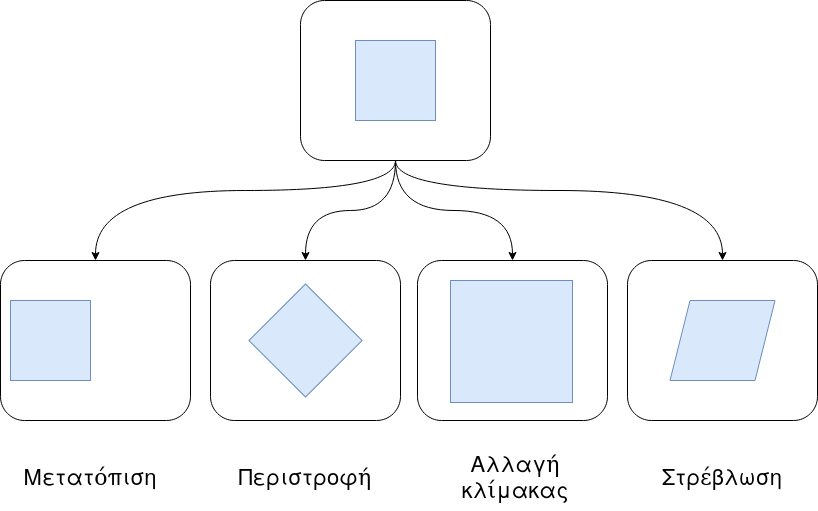
\includegraphics[width=0.7\textwidth]{affine_2}
    \captionsetup{width=0.7\textwidth}
    \caption{Μετατόπιση, περιστροφή, αλλαγή κλίμακας και στρέβλωση ενός
    τετραγώνου.}
\end{figure}

Έστω $F(x): \Omega_F \subset \R^D \mapsto \R$ η σταθερή εικόνα, $M(x): \Omega_M
\subset \R^D \mapsto \R$ η κινούμενη εικόνα και $\bm{T_{\mu}}(\bm{x}): \Omega_F
\times \R^P \mapsto \Omega_M$ παραμετροποιημένος μετασχηματισμός συντεταγμένων,
όπου $\bm{\mu} \in \R^P$ αναπαριστά το διάνυσμα των παραμέτρων του
μετασχηματισμού. Επίσης $P$ είναι ο βαθμός ελευθερίας του μετασχηματισμού.

Ο αγχίγραμμος μετασχηματισμός ορίζεται ως:

\begin{equation*}
    \bm{T_{\mu}}(\bm{x}) = \bm{A}(\bm{x} - \bm{c}) + \bm{t} + \bm{c}
\end{equation*}

Όπου $\bm{t}$ είναι το διάνυσμα μετατόπισης και $\bm{c}$ το κέντρο περιστροφής.
Επίσης, ο πίνακας $\bm{A}$ πραγματοποιεί την περιστροφή, αλλαγή κλίμακας και
στρέβλωση. Το διάνυσμα παραμέτρων $\bm{\mu}$ θα αποτελείται από τα στοιχεία
$a_{ij}$ του πίνακα $\bm{A}$ και το διάνυσμα μετατόπισης $\bm{t}$. Στις δύο
διαστάσεις ο μετασχηματισμός έχει έξι βαθμούς ελευθερίας, ενώ στις τρεις έχει
δώδεκα.

\subsubsection{Γραμμική παρεμβολή}

Κατά την διαδικασία του υπολογισμού της μετρικής αξιολόγησης της κατάτμησης
(όπως στη \ref{MSSD}), συγκρίνονται οι τιμές των αντίστοιχων σημείων της
σταθερής εικόνας και των μετασχηματισμένων της κινούμενης. Αυτά τα
μετασχηματισμένα σημεία της κινούμενης εικόνας μπορεί να μην ανήκουν στο πλέγμα
της εικόνας. Γι᾽ αυτόν τον λόγο, είναι απαραίτητη η παρεμβολή των σημείων αυτών.

Η γραμμική παρεμβολή υπολογίζει τον σταθμισμένο μέσο όρο των γειτονικών
εικονοστοιχείων, χρησιμοποιώντας την απόσταση ως το βάρος.

\subsubsection{Χώρος κλίμακας Gauss}

Ένα πρόβλημα που συναντάται όσο αυξάνεται ο χώρος αναζήτησης της κατάτμησης,
είναι ότι υπάρχουν μεγαλύτερες πιθανότητες να καταλήξει η βελτιστοποίηση σε
κάποιο τοπικό ελάχιστο, με αποτέλεσμα να μην είναι καλό το αποτέλεσμα της. Ένας
τρόπος να αυξηθεί η πιθανότητα να βρεθεί το ολικό ελάχιστο είναι να
χρησιμοποιηθεί μία ιεραρχική διαδικασία κατά την οποία η πληροφορία των εικόνων
θα αυξάνεται από τα αρχικά προς τα τελικά στάδια. 

Ο χώρος κλίμακας Gauss είναι ένας τρόπος να επιτευχθεί το παραπάνω αποτέλεσμα
\cite{scale_space:1}. Αυτή η μέθοδος χρησιμοποιεί τον πυρήνα Gauss για να
μειώσει την πληροφορία μίας εικόνας. Ο πυρήνας Gauss ορίζεται για τρεις
διαστάσεις ως:

\begin{equation*}
    g(x,y,z,t) = \frac{1} {2 \pi t} e^{\frac{-(x^2 + y^2 + z^2) }{t}}
\end{equation*}

Όπου $\sqrt{2t}$ είναι η τυπική απόκλιση του πυρήνα και $t$ το επίπεδο του χώρου
κλίμακας. Ο πυρήνας αυτός συνελίσεται με μία εικόνα ώστε να μειωθεί η πληροφορία
της. Αυτό γίνεται σε πολλαπλά ιεραρχικά στάδια, στα οποία αρχικά η τιμή του $t$
είναι μεγάλη και μειώνεται σε κάθε στάδιο. Ιδανικά με αυτήν την μέθοδο, οι
εικόνες θα έχουν ένα ελάχιστο στο αρχικό ιεραρχικό επίπεδο, το οποίο θα είναι
κοντά στο επιθυμητό ολικό ελάχιστο. Έπειτα σε κάθε στάδιο αφού αυξάνεται η
πληροφορία, το ελάχιστο ιδανικά θα τείνει όλο και πιο κοντά στο ολικό.

Στο \autoref{fig:tGauss} παρουσιάζεται η ίδια εικόνα για διάφορες τιμές του $t$.
Από το σχήμα αυτό, παρατηρείται ότι όσο αυξάνεται η τιμή του $t$ τόσο μειώνεται
και η πληροφορία στην εικόνα.

\begin{figure}[h]
    \centering

    \begin{subfigure}[b]{0.4\linewidth}
    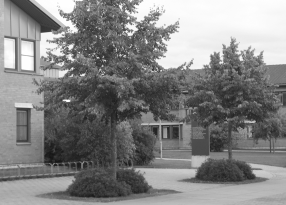
\includegraphics[width=\linewidth]{Scalespace0.png}
    \caption{$t=0$}
    \end{subfigure}
    \begin{subfigure}[b]{0.4\linewidth}
    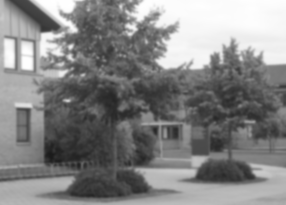
\includegraphics[width=\linewidth]{Scalespace1.png}
    \caption{$t=0.5$}
    \end{subfigure}

    \begin{subfigure}[b]{0.4\linewidth}
    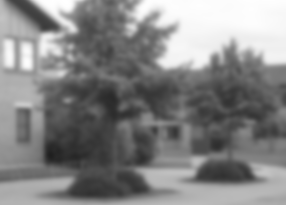
\includegraphics[width=\linewidth]{Scalespace2.png}
    \caption{$t=2$}
    \end{subfigure}
    \begin{subfigure}[b]{0.4\linewidth}
    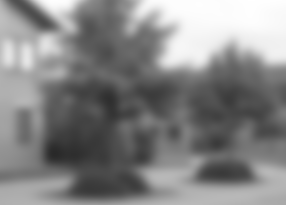
\includegraphics[width=\linewidth]{Scalespace3.png}
    \caption{$t=8$}
    \end{subfigure}

    \begin{subfigure}[b]{0.4\linewidth}
    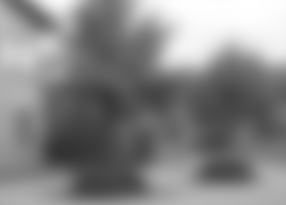
\includegraphics[width=\linewidth]{Scalespace4.png}
    \caption{$t=32$}
    \end{subfigure}
    \begin{subfigure}[b]{0.4\linewidth}
    
\includegraphics[width=\linewidth]{Scalespace5.png}
    \caption{$t=128$}
    \end{subfigure}

    \caption{Χώρος κλίμακας Gauss για διάφορες τιμές του $t$.}
    \label{fig:tGauss}
\end{figure}

\subsubsection{Δειγματοληψία συντεταγμένων εικόνας}

Κατά την διαδικασία της αξιολόγησης μπορεί να χρησιμοποιηθεί η διαδικασία της
δειγματοληψίας συντεταγμένων εικόνας ώστε να μειωθεί ο υπολογιστικός χρόνος που
χρειάζεται για την αξιολόγηση. Στην διαδικασία αυτή επιλέγονται τυχαίες
συντεταγμένες (σημεία στον χώρο της εικόνας) με ομοιόμορφη κατανομή, ώστε να
χρησιμοποιηθούν για την αξιολόγηση. Μέσω παρεμβολής των συντεταγμένων αυτών
δημιουργείται η νέα δειγματοληπτημένη εικόνα.

\subsubsection{Μάσκα εικόνας}

Αν μία εικόνα (είτε σταθερή, είτε κινούμενη) έχει περιοχές στις οποίες δεν
υπάρχουν χαρακτηριστικά ενδιαφέροντος, τότε μπορεί να χρησιμοποιηθεί μία μάσκα
εικόνας, ώστε μην να συμπεριληφθούν οι περιοχές αυτές στην διαδικασία της
κατάτμησης. Η μάσκα εικόνας είναι μία δυαδική εικόνα, η οποία υποδεικνύει εάν
ένα εικονοστοιχείο θα συμπεριληφθεί στην διαδικασία της κατάτμησης. Το μέγεθος
της μάσκας είναι ίδιο με το μέγεθος της εικόνας που θα εφαρμοστεί, ώστε να
υπάρχει αντιστοιχία μεταξύ των εικονοστοιχείων της εικόνας και των
εικονοστοιχείων της μάσκας. Επομένως, κάθε εικονοστοιχείο της μάσκας δηλώνει εάν
το αντίστοιχο εικονοστοιχείο της εικόνας θα χρησιμοποιηθεί στην κατάτμηση.

\subsection{Μέτρα αξιολόγησης}

Τα μέτρα αξιολόγησης χρησιμοποιούνται για να αξιολογήσουν το αποτέλεσμα της
κατάτμησης. Συγκρίνουν το αποτέλεσμα της κατάτμησης με το επιθυμητό αποτέλεσμα,
ούτως ώστε να παράξουν μία αριθμητική αναπαράσταση της ποιότητας της κατάτμησης.
Με αυτόν το τρόπο μπορούν να συγκριθούν διαφορετικοί αλγόριθμοι κατάτμησης και
διαφορετικές τιμές για τον ίδιο αλγόριθμο.

Η επιλογή του μέτρου ή των μέτρων αξιολόγησης έχει μεγάλη σημασία για την
δημιουργία και τον συντονισμό (επιλογή των κατάλληλων μεταβλητών) του μοντέλου
επειδή, είναι το μέτρο που θα χρησιμοποιηθεί για την επιλογή του καταλληλότερου
μοντέλου. Η επιλογή αυτή ταυτίζεται με την επιθυμητή συμπεριφορά του τελικού
μοντέλου. Για παράδειγμα, αν το επιθυμητό μοντέλο πρέπει να έχει όσο είναι
δυνατόν πιο λίγα αληθή αρνητικά, τότε πρέπει να επιλεχθεί και το ανάλογο μέτρο
αξιολόγησης που να ικανοποιεί τον περιορισμό αυτό.

\subsubsection{Συντελεστής ομοιότητας Dice}

Ο συντελεστής ομοιότητας Dice είναι μία μέτρηση που εκτιμά την ομοιότητα μεταξύ
δύο συνόλων \cite{dice:1}. Είναι γνωστός επίσης και ως δείκτης Sørensen–Dice,
συντελεστής Dice και F1 σκορ. Ο συντελεστής ομοιότητας Dice ορίζεται ως:

\begin{equation*}
    DSC = \frac{2 \abs{X \cap Y}} {\abs{X} + \abs{Y}}
\end{equation*}

Όπου $X$ και $Y$ είναι σύνολα, $\abs{x}$ είναι ο αριθμός των στοιχείων του
συνόλου $x$ και $\cap$ δηλώνει την τομή δύο συνόλων.

Στην αξιολόγηση της κατάτμησης εικόνας τα παραπάνω σύνολα αποτελούνται από το
σύνολο των εικονοστοιχείων που ανήκουν σε μία κλάση. Επομένως ο συντελεστής
αυτός υπολογίζει το ποσοστό των σημείων μίας κλάσης που επικαλύπτονται. Η
μέγιστη τιμή του συντελεστή είναι $1$ και η ελάχιστη $0$.

\subsubsection{Δείκτης δομικής ομοιότητας}

Ο δείκτης δομικής ομοιότητας \cite{SSIM:1} (Structural SIMilarity index, SSIM)
είναι μία μετρική της ομοιότητας δύο εικόνων. Χρησιμοποιεί τις σύγκρισεις της
φωτεινότητας, της αντίθεσης και της δομής των εικόνων. Κατά την δημιουργία μίας
εικόνας η φωτεινότητα των αντικειμένων της εικόνας εξαρτάται από τον φωτισμό και
την ανακλαστικότητα των αντικειμένων αυτών, αλλά και από την δομής τους. Γι᾽
αυτό τον λόγο είναι επιθυμητό να διαχωριστεί η επίδραση της φωτεινότητας έτσι
ώστε η δομή να είναι ανεξάρτητη από την φωτεινότητα. Επομένως μπορεί να οριστεί
η δομική πληροφορία της εικόνας ως τα χαρακτηριστικά των αντικειμένων της που
είναι ανεξάρτητα από την φωτεινότητα και την αντίθεση.

Η φωτεινότητα ενός σήματος ορίζεται ως:

\begin{equation}\label{luminance}
    \mu_x = \frac {1} {N} \sum_{i=1}^{N} x_i
\end{equation}

Όπου $x$ είναι το σήμα  και $N$ ο αριθμός των στοιχείων του. Αν οι τιμές των
εικονοστοιχείων μίας εικόνας τοποθετηθούν σε ένα διάνυσμα τότε μπορεί να
χρησιμοποιηθεί ο τύπος \eqref{luminance} για τον υπολογισμό της φωτεινότητας
αλλά και των παρακάτω τύπων. Για να αφαιρεθεί η επίδραση της φωτεινότητας στο
σήμα θα πρέπει να ισχύει:

\begin{equation*}
    \sum_{i=1}^{N} x_i = 0
\end{equation*}

Η αντίθεση της σήματος-εικόνας εκτιμάτε με την διακύμανση του σήματος:

\begin{equation*}
    \sigma_x = \sqrt{\left(\, \frac{1}{N-1} \sum_{i=1}^{N} {\left(\,x_i -
                     \mu_x\right)}^2\, \right)}
\end{equation*}

Για να αφαιρεθεί και η επίδραση της αντίθεσης θα πρέπει να κανονικοποιηθεί το
σήμα, δηλαδή να διαιρεθεί με την διακύμανση του ώστε να έχει μοναδιαία
διακύμανση. Επομένως

\begin{equation*}
    \hat{x} = \frac{x-\mu_x} {\sigma_x}
\end{equation*}

Όπου $\hat{x}$ είναι το κανονικοποιημένο σήμα. Η σύγκριση της φωτεινότητας δύο
εικόνων $x$ και $y$ ορίζεται ως:

\begin{equation}\label{luminance_comp}
    l(x,y) = \frac {2\mu_x\mu_y + C_1} {\mu_x^2 + \mu_y^2 + C_1}
\end{equation}

Η σταθερά $C_1$ μπορεί να χρησιμοποιηθεί για να αποφευχθεί υπολογιστική αστάθεια
για μικρές τιμές του παρανομαστή. Η σύγκριση της αντίθεσης ορίζεται ως:

\begin{equation}\label{contrast_comp}
    c(x,y) = \frac {2\sigma_x\sigma_y + C_2} {\sigma_x^2 + \sigma_y^2 + C_2}
\end{equation}

Όπου η σταθερά $C_2$ χρησιμοποιείται επίσης για την υπολογιστική σταθερότητα.
Επειδή η συσχέτιση των κανονικοποιημένων σημάτων $\hat{x}$ και $\hat{y}$ είναι
ίδια με την συσχέτιση των μη κανονικοποιημένων σημάτων, μπορεί να οριστεί η
σύγκριση της δομής (που είναι ανεξάρτητη από την φωτεινότητα και την αντίθεση)
ως:

\begin{equation}\label{structure_comp}
    s(x,y) = \frac {\sigma_{xy} + C_3} {\sigma_x \sigma_y + C_3}
\end{equation}

Όπου η σταθερά $C_3$ χρησιμοποιείται επίσης για την υπολογιστική σταθερότητα και
$\sigma_{xy}$ είναι η συνδιακύμανση των σημάτων και ορίζεται ως:

\begin{equation*}
    \sigma_{xy} = \frac {1} {N-1} \sum_{i=1}^{N} {(x_i - \mu_x) (y_i - \mu_y)}
\end{equation*}

Τέλος, χρησιμοποιώντας τις συγκρίσεις της φωτεινότητας, της αντίθεσης και της
δομής (\eqref{luminance_comp}, \eqref{contrast_comp} και \eqref{structure_comp}
αντίστοιχα), ο τύπος του δείκτης δομικής ομοιότητας ορίζεται ως:

\begin{equation*}
    SSIM(x,y) = \left[l(x,y)\right]^\alpha \left[c(x,y)\right]^\beta 
                \left[l(x,y)\right]^\gamma
\end{equation*}

Οι τιμές $\alpha$, $\beta$ και $\gamma$ χρησιμοποιούνται για να ορίσουν την
επίδραση κάθε σύγκρισης.

\subsection{Προεπεξεργασία δεδομένων}

Η προεπεξεργασία των δεδομένων αποτελεί ένα από τα πιο βασικά βήματα της
μηχανικής μάθησης. Σε αυτό το βήμα τα δεδομένα αναλύονται και επεξεργάζονται
ούτως ώστε η διαδικασία της μάθησης να είναι πιο αποτελεσματική. Αν τα δεδομένα
περιέχουν περιττές και ασυσχέτιστες πληροφορίες για το πρόβλημα που
χρησιμοποιούνται, τότε δυσκολεύουν την διαδικασία της μάθησης. Το ίδιο ισχύει
και για αφερέγγυα και θορυβώδη δεδομένα. Επίσης στην προεπεξεργασία μπορεί να
αυξηθεί η σημαντικότητα μερικών χαρακτηριστικών των δεδομένων.

Στην περίπτωση όπου τα δεδομένα είναι εικόνας-απεικονίσεις, σκοπός της
προεπεξεργασίας είναι να παραχθεί μία νέα εικόνα-απεικόνιση που θα έχει καλύτερα
αποτελέσματα στην μάθηση από αυτά της αρχικής. Πιο αναλυτικά, σκοπεύει στην
εξάλειψη της αθέμιτης διαστρέβλωσης τους, στην αύξηση της σημαντικότητας μερικών
χαρακτηριστικών της εικόνας και στον γεωμετρικός μετασχηματισμός της εικόνας
\cite{Image_preprocessing:1}.

\iffalse
Οι μέθοδοι προεπεξεργασίας
δεδομένων εικόνας μπορούν να διαχωριστούν σε τέσσερις κατηγορίες ανάλογα με την
γειτονία των εικονοστοιχείων που χρησιμοποιείται για τον υπολογισμό της νέας
εικόνας, όπως παρουσιάζεται στο \cite{Image_preprocessing:1}. Οι κατηγορίες
αυτές είναι:

\begin{enumerate}
    \item Μέθοδοι που επεξεργάζονται την ένταση κάθε εικονοστοιχείου ξεχωριστά.
    \item Γεωμετρική μετασχηματισμοί.
    \item Μέθοδοι που χρησιμοποιούν πληροφορίες των γειτονικών εικονοστοιχείων.
    \item 
\end{enumerate}
\fi

\subsubsection{Αντιστοίχιση ιστογράμματος}

Η αντιστοίχιση ιστογράμματος είναι ένας μετασχηματισμός της εικόνας κατά τον
οποίο το ιστόγραμμα της εικόνας αντιστοιχίζεται με ένα άλλο ιστόγραμμα το οποίο
μπορεί να προέρχεται από άλλη εικόνα. Αυτό μπορεί να επιτευχθεί με διάφορους
αλγόριθμους. Ο αλγόριθμος που θα παρουσιαστεί περιγραφικά παρακάτω βασίζεται στο
\cite{histogram_matching:1}.

Ο αλγόριθμος πραγματοποιεί γραμμικούς μετασχηματισμούς για διάφορα τμήματα του
ιστογράμματος των εικόνων. Αρχικά υπολογίζει τα τμήματα αυτά μέσω
προκαθορισμένων τιμών της αθροιστικής συνάρτησης κατανομής. Έπειτα υπολογίζει
για κάθε άκρο των μέσω όρο των αντίστοιχων τιμών. Τέλος μετασχηματίζει γραμμικά
τις τιμές κάθε εικόνας, για κάθε διάστημα, από το αρχικό διάστημα της εικόνας,
στο τελικό διάστημα που υπολογίστηκε με τον μέσο όρο.

Στο \autoref{fig:histogram_matching} φαίνεται η διαδικασία τους γραμμικού
μετασχηματισμού μίας εικόνας. Οι τιμές της εικόνας μετασχηματίζονται γραμμικά
από τον οριζόντιο άξονα στον κάθετο. Στο παράδειγμα αυτό υπάρχουν τέσσερα
διαστήματα, όπου $\mu_1, \mu_2, \mu_3, \mu_4$ είναι τα άκρα του αρχικού
διαστήματος και $\mu_{s1}, \mu_{s2}, \mu_{s3}, \mu_{s4}$ τα άκρα του τελικού.
$m_1, m_2$ είναι η ελάχιστη και η μέγιστη τιμή αντίστοιχα της εικόνας και
$m_{s1}, m_{s2}$ ίδια άκρα για το αποτέλεσμα της αντιστοίχισης ιστογράμματος.

\begin{figure}[ht]
    \centering
    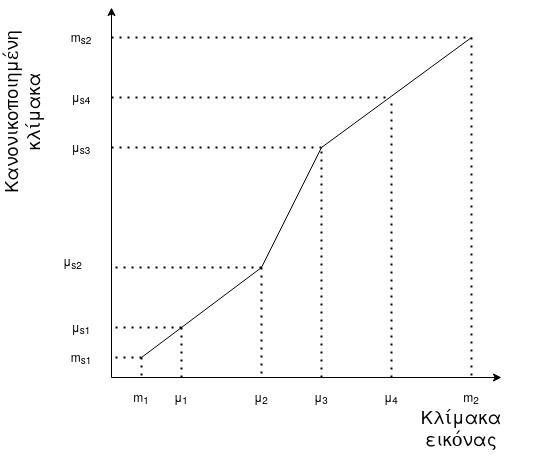
\includegraphics[width=0.6\textwidth]{histogram_matching_2}
    \iffalse
    \caption{Γραμμικός μετασχηματισμός μίας εικόνας για τέσσερα άκρα. $\mu_1,
             \mu_2, \mu_3, \mu_4$ είναι τα άκρα του αρχικού διαστήματος και
             $\mu_{s1}, \mu_{s2}, \mu_{s3}, \mu_{s4}$ τα άκρα του τελικού. $m_1,
             m_2$ είναι η ελάχιστη και η μέγιστη τιμή αντίστοιχα της εικόνας και
             $m_{s1}, m_{s2}$ ίδια άκρα για το αποτέλεσμα της αντιστοίχισης
             ιστογράμματος.}
    \fi
    % \captionsetup{width=0.7\textwidth}
    \caption{Γραμμικός μετασχηματισμός αντιστοίχισης ιστογράμματος μίας εικόνας
             για τέσσερα άκρα.}
    \label{fig:histogram_matching}
\end{figure}

\subsubsection{Απαλοιφή θορύβου εικόνας μέσω ροής της καμπυλότητας}

Η ροή της καμπυλότητας μπορεί να χρησιμοποιηθεί για την απαλοιφή του θορύβου.
Συγκεκριμένα, σε μία μία εικόνα χρησιμοποιούνται οι καμπύλες που σχηματίζονται
από τα εικονοστοιχεία που έχουν την ίδια τιμή (φωτεινότητα εικονοστοιχείου). Οι
καμπύλες αυτές εξελίσσονται \cite{curvature_flow:1} μέσω της μερικής διαφορικής
εξίσωσης:

\begin{equation*}
    I_t = \kappa \abs{\nabla I}
\end{equation*}

Όπου $I$ είναι η εικόνα και $\kappa$ η καμπυλότητα. Η καμπυλότητα μίας καμπύλης
$\bm{\gamma}$ ορίζεται ως:

\begin{equation*}
    \kappa = \frac {\norm{\bm{\gamma}' \times \bm{\gamma}''}}
                   {\norm{\bm{\gamma}'}^3}
\end{equation*}

Όπου το σύμβολο $x'$ δηλώνει την παράγωγο της συνάρτησης $x$ ως προς το χρόνο.
Επίσης $\norm{v}$ είναι η ευκλείδεια νόρμα του διανύσματος $v$.

Αυτή η τεχνική για την απαλοιφή του θορύβου έχει το πλεονέκτημα ότι διατηρεί
τα αιχμηρά όρια της εικόνας ενώ ταυτόχρονα εξομαλύνει τα υπόλοιπα σημεία. Επειδή
οι ροή των καμπυλών τείνει προς την εξάλειψη τους, η υπερβολική χρήση της
τεχνική θα οδηγήσει στη εξάλειψη της πληροφορίας στη εικόνα.

\subsection{Διασταυρωμένη επικύρωση}

Σύμφωνα με το \cite{cross_validation:1}, διασταυρωμένη επιτήρηση είναι μια
στατιστική μέθοδος αξιολόγησης και σύγκρισης των αλγορίθμων μάθησης διαιρώντας
τα δεδομένα σε δύο τμήματα. Το ένα χρησιμοποιείται για την εκμάθηση ή την
εκπαίδευση ενός μοντέλου και το άλλο χρησιμοποιείται για την επικύρωση του
μοντέλου. Ο σκοπός της διασταυρωμένης επικύρωσης είναι μέσω αυτής να αξιολογηθεί
η δυνατότητα του μοντέλου να πραγματοποιεί σωστές προβλέψεις για δεδομένα που
δεν χρησιμοποιήθηκαν για την εκπαίδευση του. Έτσι μπορεί να κριθεί η ικανότητα
του μοντέλου να γενικεύει (ικανότητα πρόβλεψης του σε ανεξάρτητα δεδομένα).

\subsubsection{Αφήνω ένα έξω διασταυρωμένη επικύρωση}

Η μέθοδος αφήνω ένα έξω διασταυρωμένης επικύρωσης είναι μία μέθοδος
διασταυρωμένης επικύρωσης κατά την οποία χρησιμοποιείται μία παρατήρηση από το
σύνολο των δεδομένων για την επικύρωση του μοντέλου και οι υπόλοιπες για την
εκπαίδευση του. Η διαδικασία αυτή επαναλαμβάνεται μέχρις ότου κάθε παρατήρηση
του συνόλου δεδομένων έχει χρησιμοποιηθεί για την επικύρωση. Αν $\bm{m}$ είναι ο
συνολικός αριθμός των παρατηρήσεών, τότε η διαδικασία αυτή επαναλαμβάνεται
$\bm{m}$ φορές.



%TODO: μία εικόνα, μεταβλητές και περιγραφή τους


\iffalse
NOTES:
    !Graph-Based Framework for Label Fusion 
    !lasso
    !registration
    !dice, (maybe) sse
    !structural similarity measure (SSIM)
    !φιλτρα
    !leave-one-out cross validation
\fi

\newpage

%TODO: βιβλιογραφία στα περιεχόμενα
\printbibliography


\end{document}
